\chapter{ブロックとOCamlコードとの相互変換}\label{chap:converter}


本節では,ブラウザ上でのブロックとOCamlコードの相互変換の実現について説明する.
組み立てられたブロックからOCamlコードを生成することで,
本来のテキストによるOCamlプログラミングへのイメージが湧きやすくなる.
逆にOCamlコードからブロックへの変換を実現することで,
型や変数の束縛関係を視覚的に確認できることになり,
テキストベースのプログラミングに移行しつつある初学者にとっての補助となることが期待できる.
また, OCaml コードから複雑なブロックの組み合わせを復元できるので,
OCaml Blocklyの開発時に,
特定の条件下のUI/UXをテストしたいときに使うこともできる.
双方向の変換について,それぞれ説明を行う.

\section {ブロックからOCamlコードへ}
第\ref{sec:hajimeni}節で述べた通り,
Blocklyは標準のブロックに対してJavaScriptやPythonなどのスクリプト言語へのコード生成をサポートしている.
それらの実装と同じような手順で,
本研究で新たに追加したOCamlブロックに対するOCamlコードの生成を実装した.
ブロックは構文木と一対一対応しているので,
OCamlコードへの変換は比較的自明である.
% デザインレシピをともに出力する。
\section {OCamlコードからブロックへ}
%まだ実験的な実装だけど.
第\ref{impl:osunaba}節で述べた通り,BlocklyはブロックとXMLのエンコード,
デコードをサポートしている.
つまり,OCamlコードをブロック表現のXMLに変換することができれば,
ブロックを生成することができる.
OCamlコードをパーズするために,
OCamlコンパイラのパッケージcompiler-libsを利用した.
入力されたOCamlコードからcompiler-libs によって抽象構文木を得たのちは,
木をトラバースして対応するブロックの XMLを組み立てる.
これらをビルドしたものをjs\_of\_ocamlでJavaScriptへと変換すれば,
ブラウザ上でOCamlコードからブロックへの変換が実現できる.
変換するコードの例を図\ref{OCamlWallis}に,
コードをブロックに変換したものを図\ref{fig:piOCaml}に示す.

\begin{figure}[h]
\centering
\begin{verbatimtab}[2]
let rec pi_impl n d =
  if n > 0.0
  then n *. n /. d /. (d -. 2.0) *. pi_impl (n -. 2.0) (d -. 2.0)
  else 1.0;;
let pi n = 2.0 *. pi_impl (n *. 2.0) (n *. 2.0 +. 1.0);;
let pi_exp = pi 9000.
\end{verbatimtab}
\vspace{-2.0zh}
\caption{ウォリス積を利用して円周率を計算する OCaml プログラム\label{OCamlWallis}}
\vspace{0.6zh}

 \centering
 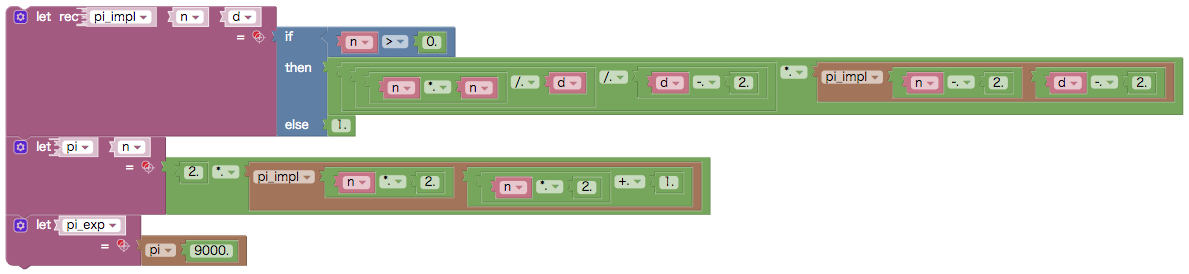
\includegraphics[keepaspectratio, scale=0.4]{img/pi.png}
 \caption{図\ref{OCamlWallis}に現したウォリス積を利用したOCamlプログラムをブロックに自動で変換したもの.
型の整合性,変数束縛ともに反映されている.\label{fig:piOCaml}}
\end{figure}
